Systematic uncertainties treatment for \ZZ\ analysis is similar to the
\WW\ one. This section describes only systematic effects that are
different from \WW{}.

\subsection{\WZ\ and \ZZ\ background}

$\wz$ and $\zz$ background are the ireducible background to the 
Higgs $\to$ \ZZ\  search. We do not have a data-driven estimate yet, 
therefore the shapes are taken from MC. 
Similar to the \WW{} background treatment as in the $\hww$ analysis, 
we accounts for the effects due to the therorectical uncertainties. 
We compare the default shape simulated with the Pythia generator with an alternative generator, which was taken as the one sigma 
variation histogram. In this case, we only have the MC sample form Madgraph. 

The $\wz$ background shape can be further validated with data in a control 
region of events with 3 leptons with increasing luminosity. 
For the $\zz$ background we reweight the $\pt$ spectrum of Z to the NLO 
prediction by applying the event-by-event kfactors computed from MCFM. 
To assess the QCD scale variations to the shape, we can 
compute the event-by-event k-factor with the normalization and 
factorization scales independently. 
       

\subsection{Top and \WW\   Background}

For the Top and \WW{} background involving the $\mu^+\mu^-$, $e^+\mu^-$ and 
$e^+e^-$ that occur with equal rates ( after correcting the electron 
to muon efficiency ratio), we can estimate the shapes from data using 
the opposite flavor ($e^\pm\mu^\mp$ states. To ensure the kinematics 
in the opposite flavor states to be the same as in the same flavors, we 
need to apply the same selections in the signal region. The 
statistics is rather limited after the $\met$ preselections and 
b-tagging veto as shown in Fig.~\ref{fig:mtemdatamc}. 

The top background statisitcs can be enriched by relaxing the btag requirement 
in all the dilepton final states. We define this as the control region 
to study the top event shape. Figure~\ref{fig:mtcompsigcontrl} 
compares the $m_T$ distributions between the same flavor signal region and 
the control region and found the two regions give consistent spectrum. 
Therefore we can use the data in the control region to derive the top 
shape and place the shapes in the signal region derived from MC as the 
alternative. Figure~\ref{fig:mtdatamcl} shows the comparison of the $m_T$ 
distributions between the signal MC region and the control region in both data and MC. 


Seperating the top background, the \WW{} background shape variations can be assessed 
in the same way as in the $\hww$ analysis described in the previous section.


%%%%%%%%%%%%%%
\begin{figure}[!htbp]
\begin{center}
\subfigure[]{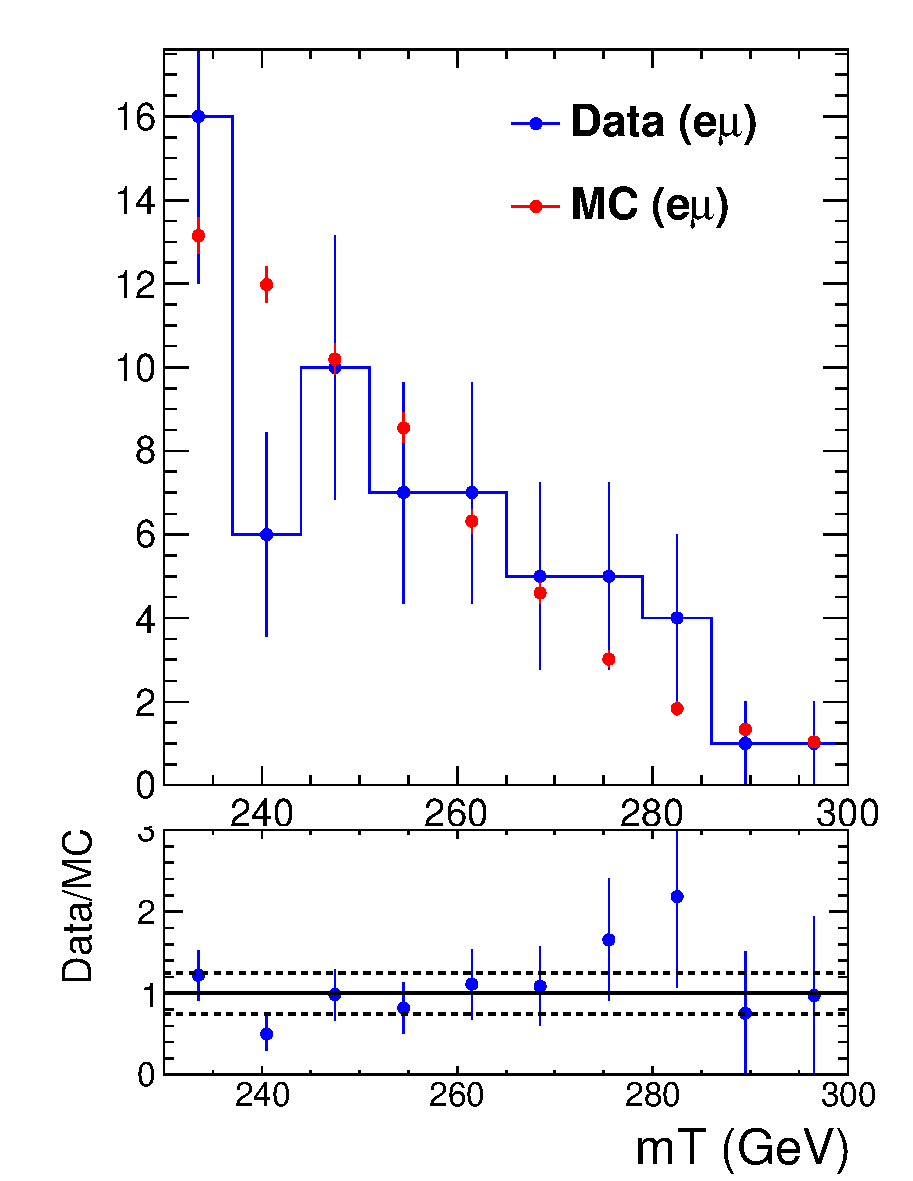
\includegraphics[width=0.49\textwidth]{figures/OF_mT_mH250_datamc_lin.pdf}}
\label{fig:mtemdatamc}
\caption{Comparing the $m_T$ transverse mass distribution in the opposite flavor between data and MC.The data corresponds to 1.1/fb.}
\end{center}
\end{figure}
%%%%%%%%%%%%%%

%%%%%%%%%%%%%%
\begin{figure}[!htbp]
\begin{center}
\begin{tabular}{cc}
\subfigure[]{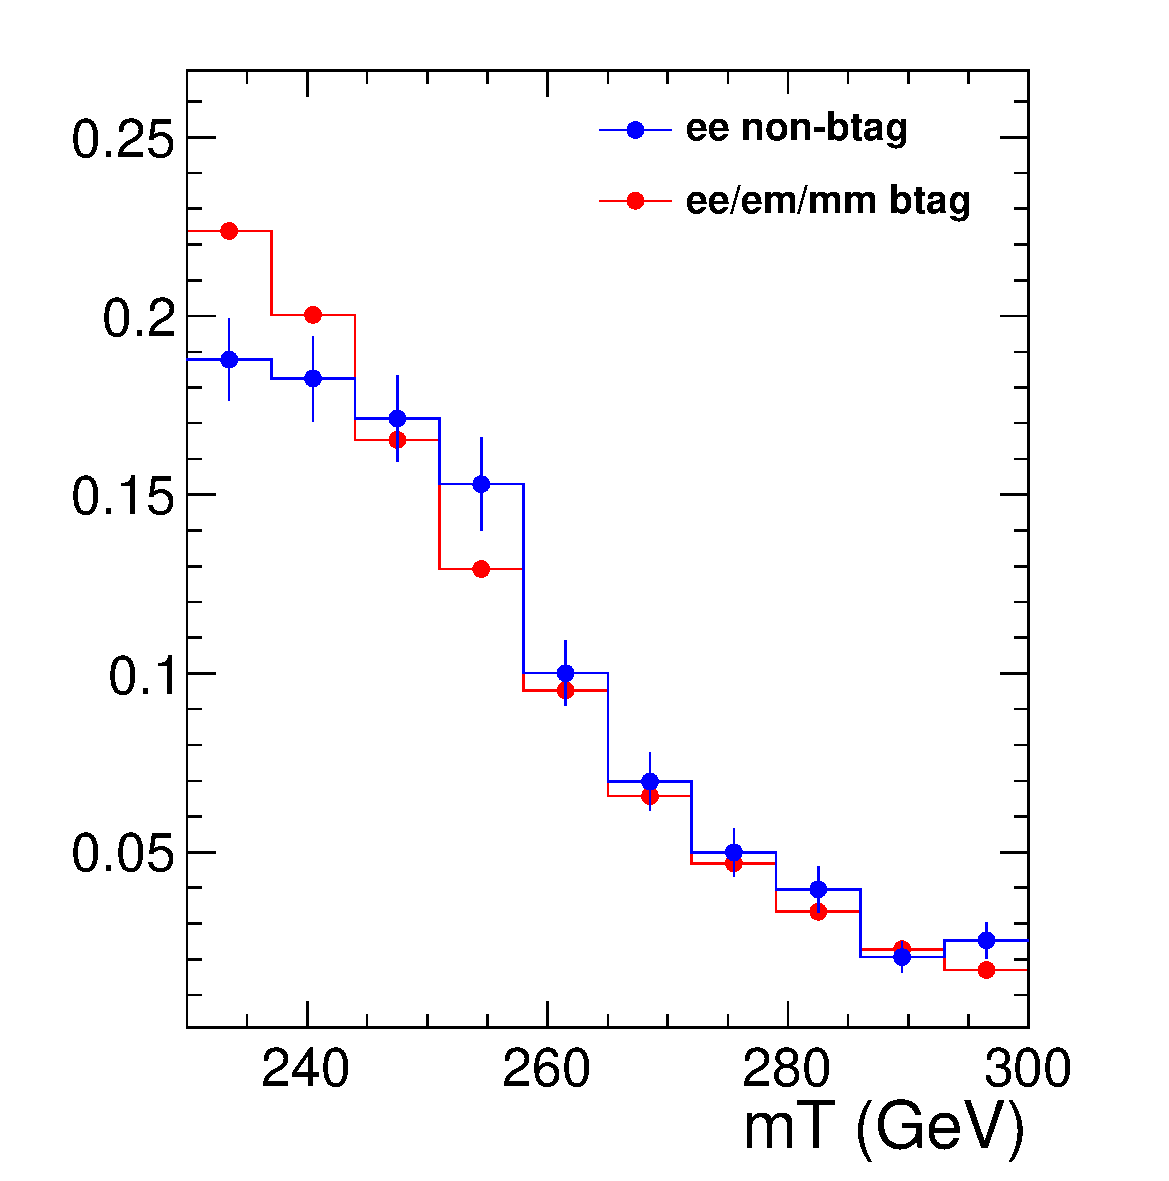
\includegraphics[width=0.49\textwidth]{figures/Top_mT_mH250_ee_lin.pdf}}
\subfigure[]{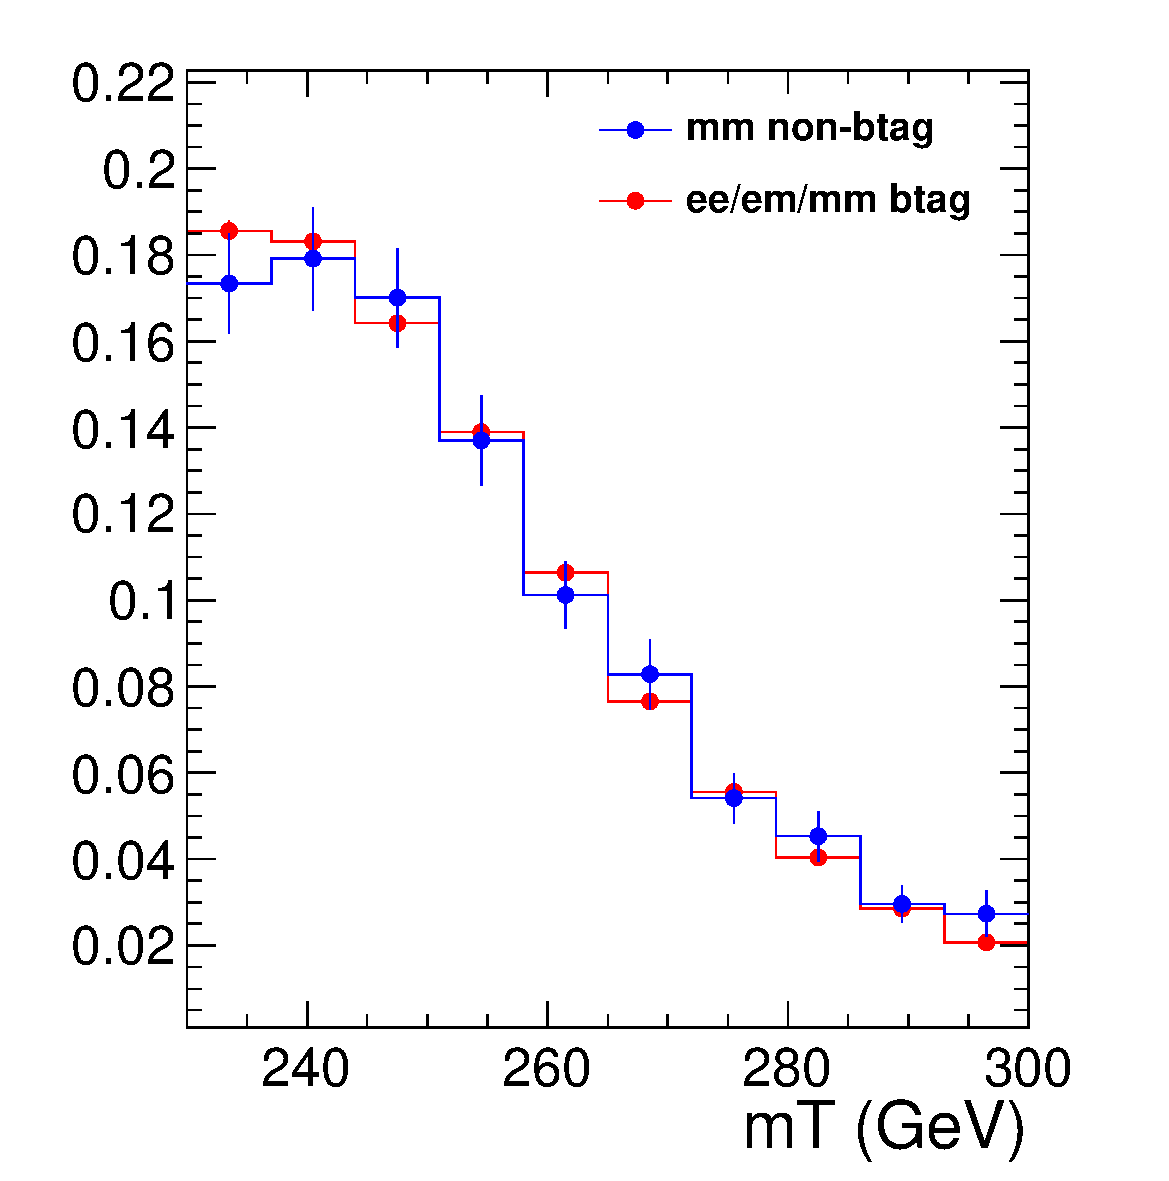
\includegraphics[width=0.49\textwidth]{figures/Top_mT_mH250_mm_lin.pdf}}\\
\end{tabular}
\label{fig:mtcompsigcontrl}
\caption{Comparing the mT distribution in the $H\to ZZ$ signal region and the top enriched control region in $ee/\mu\mu$ final states. This is evaluated with the $mH=250$ selections. }
\end{center}
\end{figure}
%%%%%%%%%%%%%%

%%%%%%%%%%%%%%
\begin{figure}[!htbp]
\begin{center}
\begin{tabular}{cc}
\subfigure[]{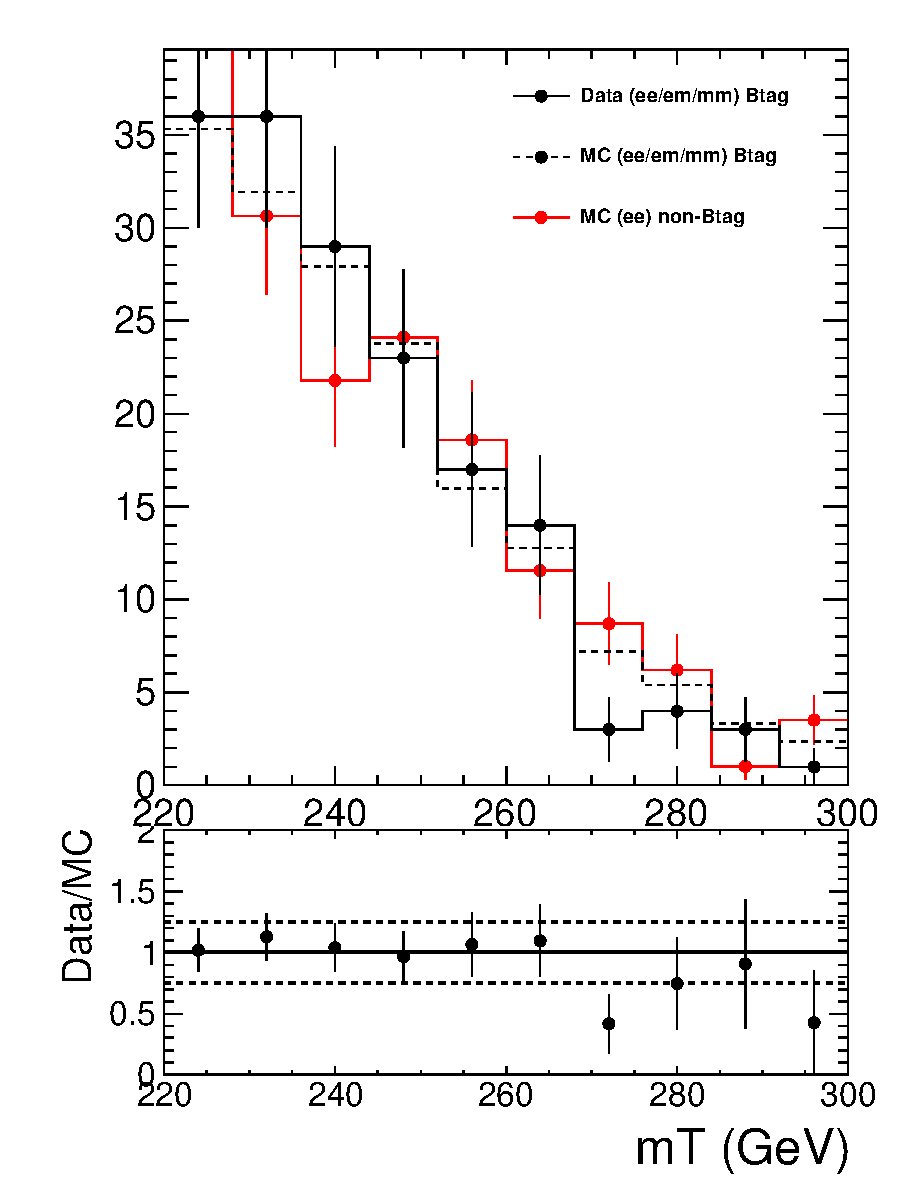
\includegraphics[width=0.49\textwidth]{figures/Top_mT_mH250_datamc_ee_lin.pdf}}
\subfigure[]{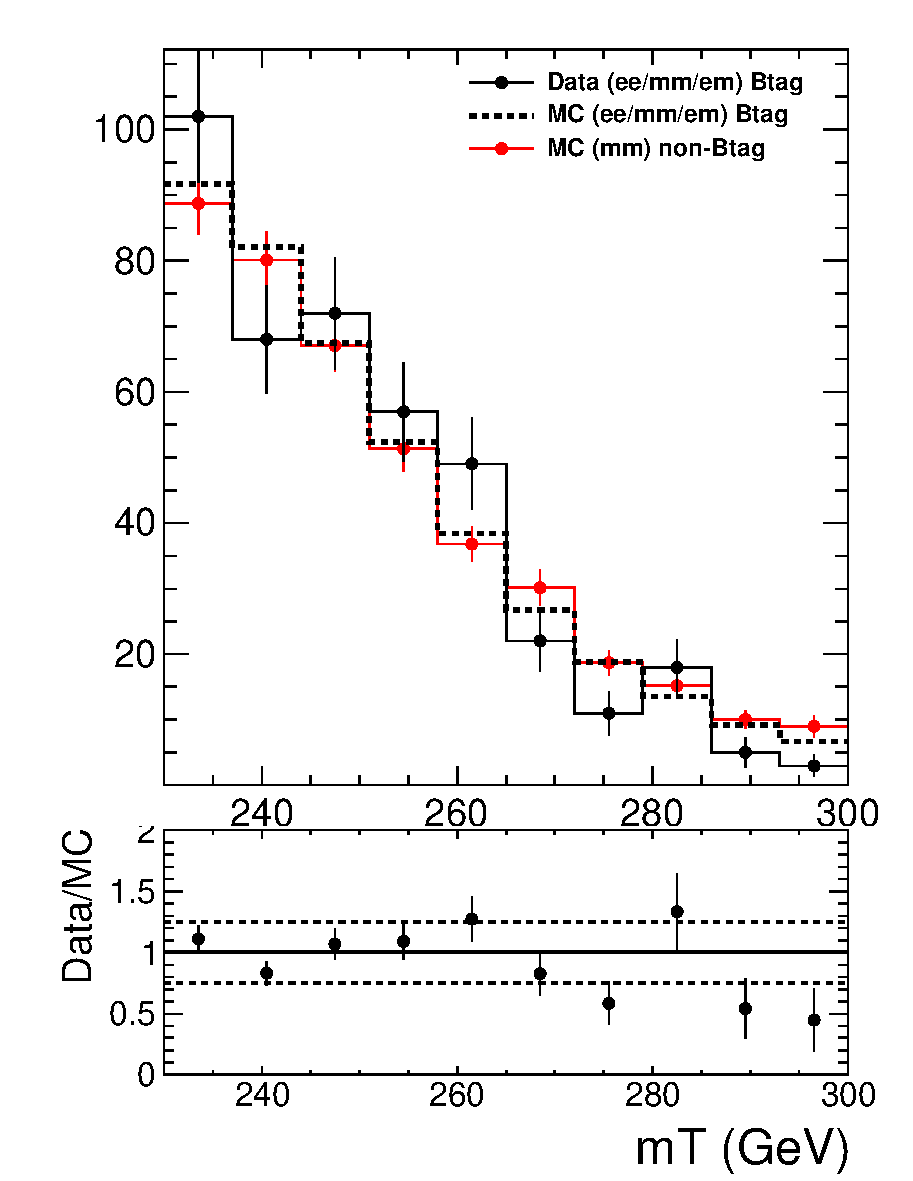
\includegraphics[width=0.49\textwidth]{figures/Top_mT_mH250_datamc_mm_lin.pdf}}\\
\end{tabular}
\label{fig:mtdatamcl}
\caption{Comparing the mT distribution in the $H\to ZZ$ signal region in MC in $ee$ (left) and $\mu\mu$ (right) and the top enriched control region in all dilepton final states requiring btagging. This is evaluated with the $mH=250$ selections. }
\end{center}
\end{figure}
%%%%%%%%%%%%%%

\subsection{\dyll\  Background}

The \dyll\  background shape can be estimated from data in the $m_T$ and BDT based 
shape analysis. This is because in both method we only use the dilepton momentum 
instead of the individual lepton information as in the matrix element method. 
The intrinsic difference between the photon jet and Z jets events are 
accounted for in the overal normalization uncertainty.
%To be more conservative, we can use the statistically limited shape in the signal region in MC as 
%the alternative shape to interpreted as the one sigma variation. 




